\documentclass[12pt]{ctexart}
\CTEXsetup[format={\Large\bfseries}]{section}
\usepackage{graphicx}
\usepackage{geometry}
\usepackage{fancyhdr}
\pagestyle{fancy}                                              
\fancyhead{} %clear all fields                                 
\pagestyle{empty}
\usepackage{amsmath}
\usepackage{amsfonts}
\usepackage{amssymb}
\usepackage{color}
\usepackage{multirow}
\usepackage{extarrows}
\usepackage{float}
\usepackage{makecell,multirow,diagbox}
\makeatletter  
\newif\if@restonecol  
\makeatother  
\let\algorithm\relax  
\let\endalgorithm\relax  
\usepackage[linesnumbered,ruled,vlined]{algorithm2e}{  
\usepackage{algpseudocode}  
\usepackage{amsmath}  
\renewcommand{\algorithmicrequire}{\textbf{Input:}}  % Use Input in the format of Algorithm  
\renewcommand{\algorithmicensure}{\textbf{Output:}} % Use Output in the format of Algorithm   
\geometry{left = 1cm, right = 1cm, top = 1.0cm, bottom = 1.8cm}
\newcommand{\eqdef}{\xlongequal{\text{def}}}%
\begin{document}
	
\author{敖睿成}
\title{应用数学导论大作业}\date{}
\maketitle

\section{摘要}
考虑方程
$$\left\{
\begin{aligned}
&\frac{\partial u}{\partial t} = \Delta u\\
&\mbox{边值条件} \\
\end{aligned}
\right.$$
本次实验中,依次针对一维情形,$ \Omega = [0,1]\times [0,1]$,L-型区域上的泊松问题上的泊松问题,分别使用有限元方法,和中心差分方法求解方程,并给出相关理论分析和实验结果。

\section{一维自适应有限元方法}
对一维问题
$$\left\{
\begin{aligned}
&-u'' = f\indent \Omega = (0,L) \\
& u'(0) =\kappa_0(u(0)-g_0) \\
& u'(L) = \kappa_L(u(L)-g_L)\\
\end{aligned}
\right.$$
对于$N+1$个结点$x_0=0,x_1 = \frac{L}{N},...x_N=L,$在子区间$[x_{i-1},x_{i+1}](i=1,2,...,N-1)$上取分段线性函数:
$$\phi_i(x)=\left\{
\begin{aligned}
&\frac{x-x_{i-1}}{h_i},\indent x\in[x_{i-1},x_i]\\
&\frac{x_{i+1}-x}{h_{i+1}},\indent x\in [x_i,x_{i+1}] \\
&0,	\indent 其他
\end{aligned}
\right.$$其中$h_i=x_i-x_{i-1},$对于边界两个结点,考虑$x_0,x_1;x_{N-1},x_N$对应的两个两点线性插值函数,这样得到$N+1$个基函数$\phi_0,\phi_1,...,\phi_N,$现求解$v(x)= \sum_{j=0}^{N}u_j\phi_j(x)$,使得
$$ -\int_{0}^{1}u''(x)v(x)dx = \int_{0}^{1}f(x)v(x)dx $$
成立,通过变分方法得到:
$$\left\{
\begin{aligned}
 -\frac{u_{i-1}}{h_i}+(\frac{1}{h_i}+\frac{1}{h_{i+1}})u_i-\frac{u_{i+1}}{h_{i+1}} &= \int_{x_{i-1}}^{x_{i+1}}f\phi'(x)dx \indent i=1,2,...,N-1\\
(\frac{1}{h_1}+\kappa_0)u_0-\frac{u_1}{h_1} &= f_0 \\
(\frac{1}{h_N}+\kappa_L)u_N-\frac{u_{N-1}}{h_N} &= f_N \\
\end{aligned}
\right.
$$
令$a_i = \frac{1}{h_i}+\frac{1}{h_{i+1}},i=1,2,...,N-1,$
$$
A = 
\begin{pmatrix}
\frac{1}{h_1}+\kappa_0 & -\frac{1}{h_1}\\
-\frac{1}{h_1}& a_1& -\frac{1}{h_2} \\
& -\frac{1}{h_2}& a_2 & \ddots \\
& & \ddots & \ddots & -\frac{1}{h_{N}}\\
& & & -\frac{1}{h_{N}} & \frac{1}{h_N}+\kappa_L 
\end{pmatrix}
$$
得到方程$$Au = F$$。分别应用均匀剖分和自适应方法,在总点数$N=10,20,80$时得到如下结果:\\
$\kappa_0=10^6,k_1=0,g_0=0,f(x)=e^{-100(x-0.5)^2}$时,\\
\begin{figure}[H]
	\centering
	\begin{minipage}[t]{0.48\textwidth}
		\centering
		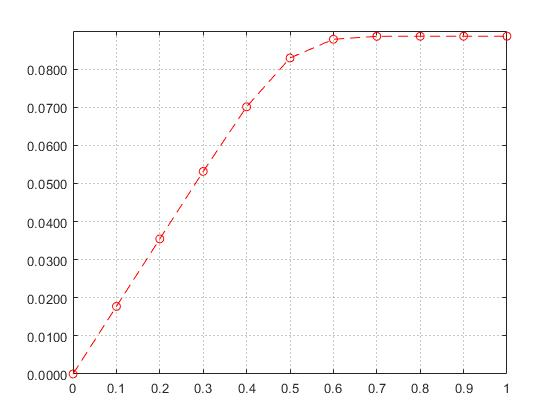
\includegraphics[width=9cm]{方程一,均匀剖分10.jpg}
		\caption{均匀剖分10}
	\end{minipage}
	\begin{minipage}[t]{0.48\textwidth}
		\centering
		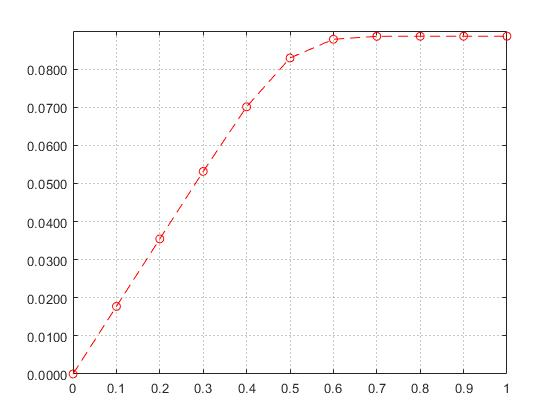
\includegraphics[width=9cm]{方程一,自适应10.jpg}
		\caption{自适应10}
	\end{minipage}
\end{figure}
\begin{figure}[H]
	\centering
	\begin{minipage}[t]{0.48\textwidth}
		\centering
		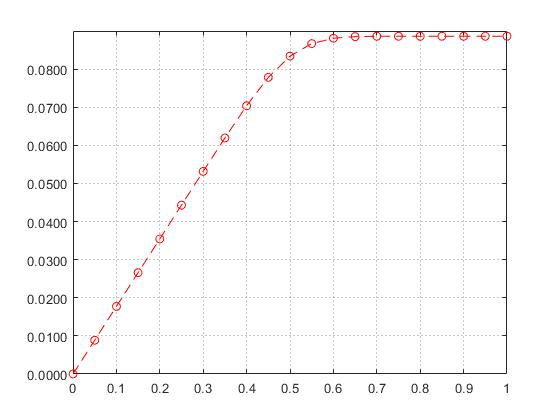
\includegraphics[width=9cm]{方程一,均匀剖分20.jpg}
		\caption{均匀剖分20}
	\end{minipage}
	\begin{minipage}[t]{0.48\textwidth}
		\centering
		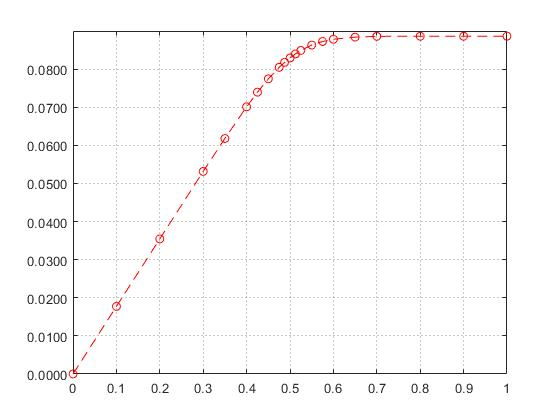
\includegraphics[width=9cm]{方程一,自适应20.jpg}
		\caption{自适应20}
	\end{minipage}
\end{figure}
\begin{figure}[H]
	\centering
	\begin{minipage}[t]{0.48\textwidth}
		\centering
		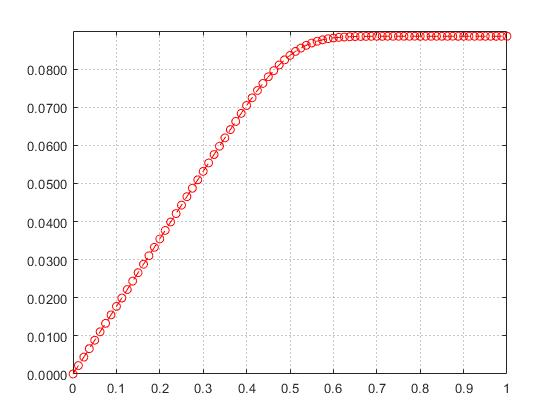
\includegraphics[width=9cm]{方程一,均匀剖分80.jpg}
		\caption{均匀剖分80}
	\end{minipage}
	\begin{minipage}[t]{0.48\textwidth}
		\centering
		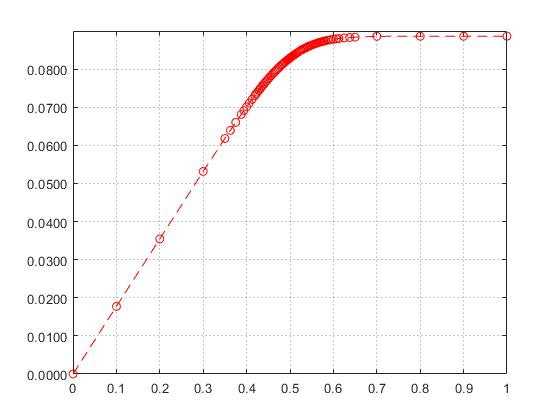
\includegraphics[width=9cm]{方程一,自适应80.jpg}
		\caption{自适应80}
	\end{minipage}
\end{figure}
$\kappa_0=10^6,k_1=10^5,g_0=0,g_L=0,f(x)=e^{-100(x-0.5)^2}$时,\\
\begin{figure}[H]
	\centering
	\begin{minipage}[t]{0.48\textwidth}
		\centering
		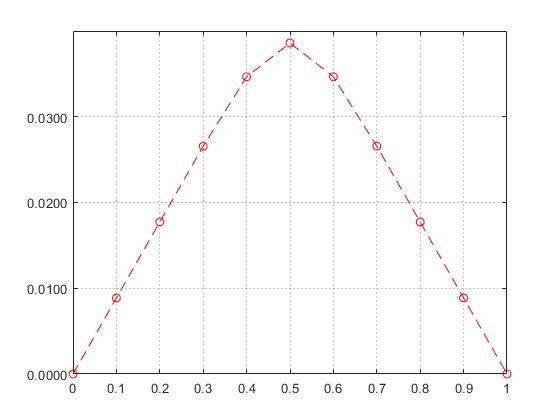
\includegraphics[width=9cm]{方程二,均匀剖分10.jpg}
		\caption{均匀剖分10}
	\end{minipage}
	\begin{minipage}[t]{0.48\textwidth}
		\centering
		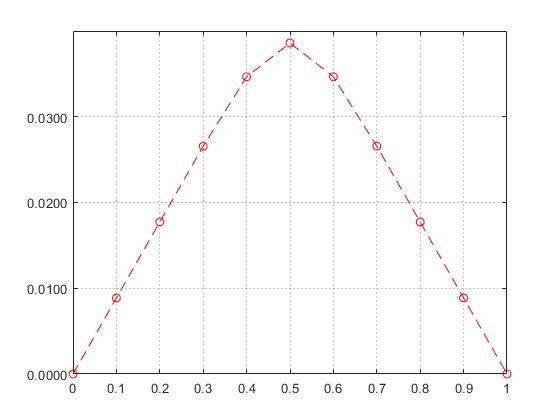
\includegraphics[width=9cm]{方程二,自适应10.jpg}
		\caption{自适应10}
	\end{minipage}
\end{figure}
\begin{figure}[H]
	\centering
	\begin{minipage}[t]{0.48\textwidth}
		\centering
		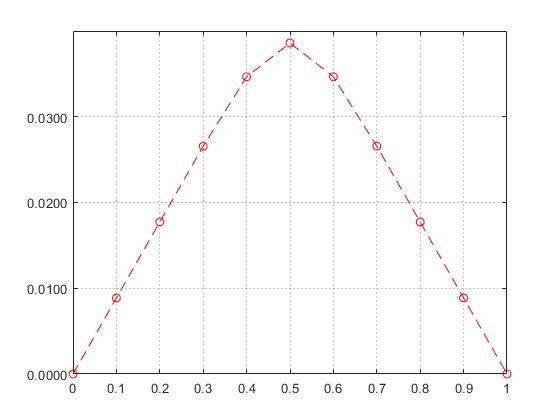
\includegraphics[width=9cm]{方程二,均匀剖分10.jpg}
		\caption{均匀剖分20}
	\end{minipage}
	\begin{minipage}[t]{0.48\textwidth}
		\centering
		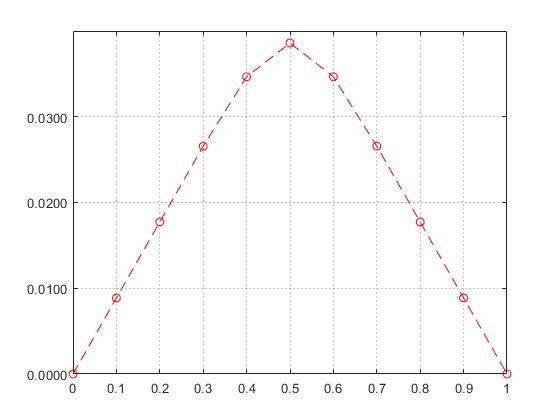
\includegraphics[width=9cm]{方程二,自适应10.jpg}
		\caption{自适应20}
	\end{minipage}
\end{figure}
\begin{figure}[H]
	\centering
	\begin{minipage}[t]{0.48\textwidth}
		\centering
		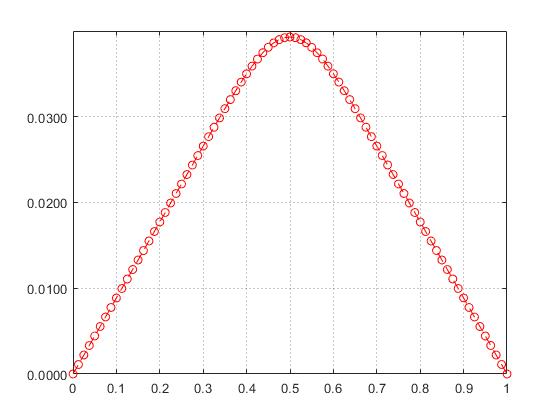
\includegraphics[width=9cm]{方程二,均匀剖分80.jpg}
		\caption{均匀剖分80}
	\end{minipage}
	\begin{minipage}[t]{0.48\textwidth}
		\centering
		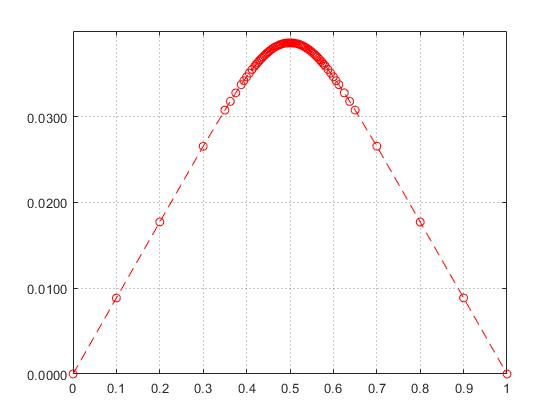
\includegraphics[width=9cm]{方程二,自适应80.jpg}
		\caption{自适应80}
	\end{minipage}
\end{figure}
$\kappa_0=10^6,k_1=0,g_0=-1,f(x)=e^{-100(x-0.5)^2}$时,\\
\begin{figure}[H]
	\centering
	\begin{minipage}[t]{0.48\textwidth}
		\centering
		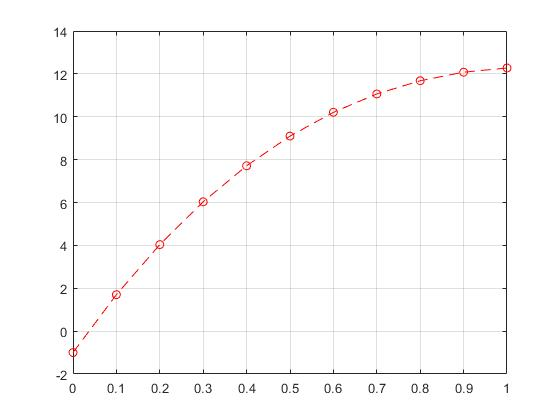
\includegraphics[width=9cm]{方程三,均匀剖分10.jpg}
		\caption{均匀剖分10}
	\end{minipage}
	\begin{minipage}[t]{0.48\textwidth}
		\centering
		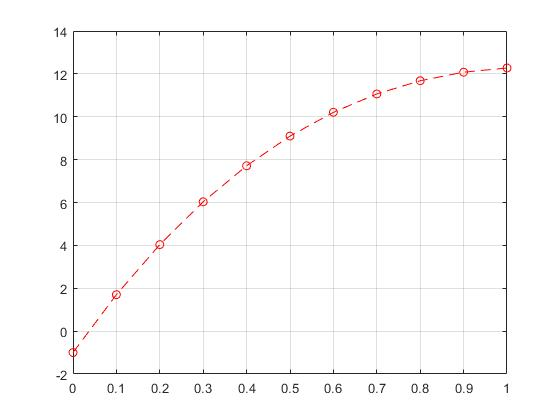
\includegraphics[width=9cm]{方程三,自适应10.jpg}
		\caption{自适应10}
	\end{minipage}
\end{figure}
\begin{figure}[H]
	\centering
	\begin{minipage}[t]{0.48\textwidth}
		\centering
		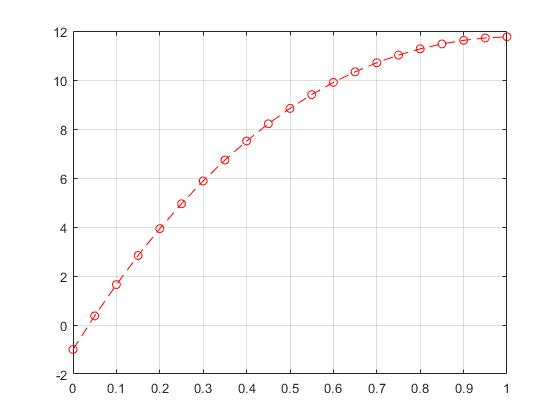
\includegraphics[width=9cm]{方程三,均匀剖分20.jpg}
		\caption{均匀剖分20}
	\end{minipage}
	\begin{minipage}[t]{0.48\textwidth}
		\centering
		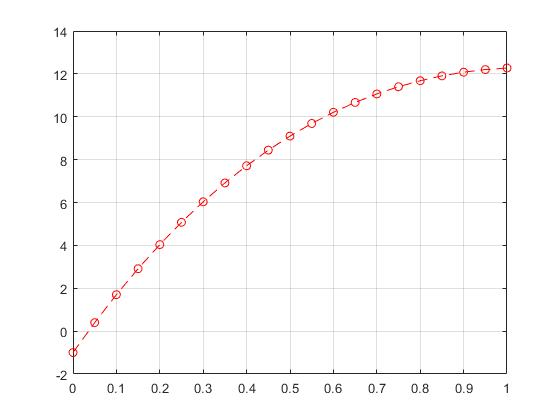
\includegraphics[width=9cm]{方程三,自适应20.jpg}
		\caption{自适应20}
	\end{minipage}
\end{figure}
\begin{figure}[H]
	\centering
	\begin{minipage}[t]{0.48\textwidth}
		\centering
		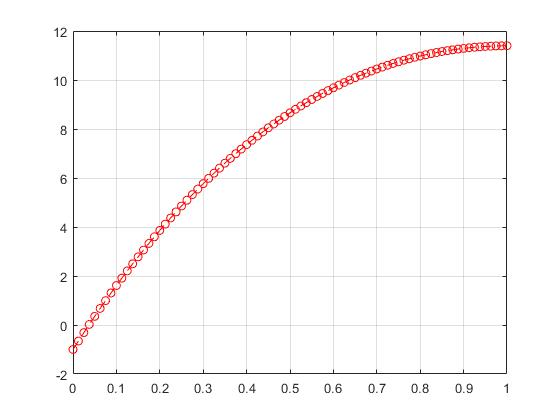
\includegraphics[width=9cm]{方程三,均匀剖分80.jpg}
		\caption{均匀剖分80}
	\end{minipage}
	\begin{minipage}[t]{0.48\textwidth}
		\centering
		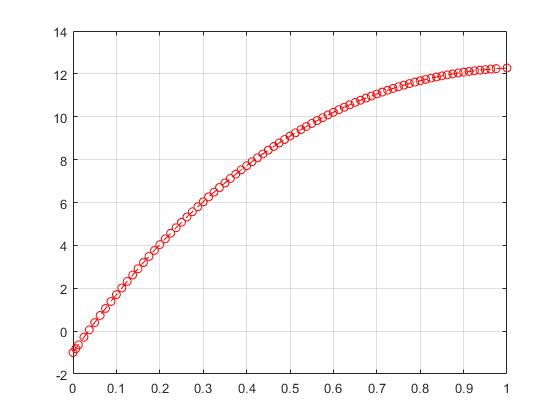
\includegraphics[width=9cm]{方程三,自适应80.jpg}
		\caption{自适应80}
	\end{minipage}
\end{figure}
可以看到,相比较均匀剖分,自适应方法在曲率大的点附近加密得较细,所得函数也更为平滑。
\section{正方形区域泊松方程}
\subsection{问题}
考虑热传导方程:
$$
\left\{
\begin{aligned}
&\frac{\partial u}{\partial t} = \Delta u\\
&u|_{\partial \Omega\times[0,1]} = 0, \Omega = [0,1]\times [0,1]\\
&u|_{t=0}=\sin(\pi x)\sin(\pi y)
\end{aligned}
\right.
$$
它有解析解$u = e^{-2\pi^2t}\sin(\pi x)\sin(\pi y)$,我们使用不同数值方法计算方程近似解,并给出相关分析。
\subsection{稳定性分析}
考察Laplace算子$$\Delta = \frac{\partial^2}{\partial x^2} + \frac{\partial^2}{\partial y^2}$$,我们使用中心差分方法
$$
L_{h_x,h_y}U_{i,j}^m \eqdef \frac{U_{i-1,j}^m-2U_{i,j}^m+U_{i+1,j}^m}{h_x^2} + \frac{U_{i,j-1}^m-2U_{i,j}^m+U_{i,j+1}^m}{h_y^2}
$$

这里$h_x,h_y$为对应分量的区间步长,对于$\frac{\partial u}{\partial t}$,我们使用一阶向前差分方法:
$$
D_k U_{i,j}^m \eqdef \frac{U_{i,j}^{m+1}-U_{i,j}^m}{k}
$$
这里$k$为时间步长。现在考虑等式:
$$
(1-\theta)L_{h_x,h_y}U_{i,j}^m+\theta L_{h_x,h_y}U_{i,j}^{m+1} = D_kU_{i,j}^m
$$
当$\theta = 1$时,为隐式格式,$\theta=0.5$时,为Crank-Nicolson格式,$\theta=0$时,为显式格式。令
$$\tilde{U} = u\left(ih_x,jh_y,\left(m+\frac{1}{2}\right)k\right)$$
应用Taylor公式,可以得到
$$
\begin{aligned}
L_{hx,hy}U_{i,j}^m =& \tilde{U}_{xx} + \tilde{U}_{yy} + \frac{2}{3!}\left(3\tilde{U}_{txx}\left(-\frac{1}{2}k\right)+3\tilde{U}_{tyy}\left(-\frac{1}{2}k\right)\right) \\
&+\frac{2}{4!}\left(\tilde{U}_{xxxx}h_x^2+\tilde{U}_{yyyy}h_y^2\right)+O(k^2+h_x^4+h_y^4)
\end{aligned}
$$
$$
\begin{aligned}
L_{hx,hy}U_{i,j}^{m+1} =& \tilde{U}_{xx} + \tilde{U}_{yy} + \frac{2}{3!}\left(3\tilde{U}_{txx}\frac{1}{2}k+3\tilde{U}_{tyy}\frac{1}{2}k\right) \\
&+\frac{2}{4!}\left(\tilde{U}_{xxxx}h_x^2+\tilde{U}_{yyyy}h_y^2\right)+O(k^2+h_x^4+h_y^4)
\end{aligned}
$$
从而有:
$$
\begin{aligned}
(1-\theta)L_{h_x,h_y}U_{i,j}^m+\theta L_{h_x,h_y}U_{i,j}^{m+1} - \Delta \tilde{U} =& \left(\left(\theta - \frac{1}{2}\right)k+\frac{h_x^2}{12}\right)\tilde{U}_{xxxx}+\left(\left(\theta - \frac{1}{2}\right)k+\frac{h_y^2}{12}\right)\tilde{U}_{yyyy}\\
&+\left(2\theta - 1\right)k\tilde{U}_{xxyy} + O(k^2+h_x^4+h_y^4)
\end{aligned}
$$
从而
$$
\begin{aligned}
(1-\theta)L_{h_x,h_y}U_{i,j}^m+\theta L_{h_x,h_y}U_{i,j}^{m+1} - \Delta \tilde{U} =& \left(\left(\theta - \frac{1}{2}\right)k+\frac{h_x^2}{12}\right)\tilde{U}_{xxxx}+\left(\left(\theta - \frac{1}{2}\right)k+\frac{h_y^2}{12}\right)\tilde{U}_{yyyy}\\
&+\left(2\theta - 1\right)k\tilde{U}_{xxyy} + O(k^2+h_x^4+h_y^4)
\end{aligned}
$$
这样截断误差$E$满足
$$
E = 
\begin{cases}
O(k^2+h_x^2+h_y^2) & \theta = 0.5\\
O(k+h_x^2+h_y^2) & \theta \neq 0.5
\end{cases}
$$
可以看出,C-N方法具有较高的截断误差阶数,现在考虑Fourier函数
$$U_{j,k}^m =\lambda_{\alpha}^me^{i(\alpha_xx_j+\alpha_yy_k)},\quad \alpha = (\alpha_x, \alpha_y)$$
解得
$$
\lambda_k = \frac{1 - 4(1-\theta)\left(\mu_x\sin^2(\alpha_xh_x/2)+\mu_y\sin^2(\alpha_yh_y/2)\right)}{1+4\theta\left(\mu_x\sin^2(\alpha_xh_x/2)+\mu_y\sin^2(\alpha_yh_y/2)\right)}
$$
因此,我们有稳定性条件

$$
\left\{
\begin{aligned}
	2(\mu_x+\mu_y)(1-2\theta) \le 1  \indent&0 \le \theta < 1/2\\
	\mbox{无条件收敛} \indent \indent  &1/2 \le \theta \le 1
\end{aligned}
\right.
$$
这表明当$h_x = h_y =h$时,对于显式格式,我们需要选取$\mu < \frac{1}{4}$,即$1/h \ge 1/4k$,才能得到收敛结果。
\subsection{数值实验}
考虑由中间$(N-1)\times(N-1)$个点,其中$N=\frac{1}{h}$为单元网格长,则对应的差分矩阵
$$
\L_h = 
\begin{pmatrix}
A_h & I_{N-1}/h\\
I_{N-1}/h^2 & A_h & I_{N-1}/h^2 \\
& I_{N-1}/h^2 & A_h & \ddots \\
& & \ddots & \ddots & I_{N-1}/h^2\\
& & & I_{N-1}/h^2 & A_h
\end{pmatrix}
$$
$$
A_h = 
\begin{pmatrix}
-2/h^2-2/h^2 & 1/h^2\\
1/h^2 & -2/h^2-2/h^2 & 1/h^2 \\
& 1/h^2 & -2/h^2-2/h^2 & \ddots \\
& & \ddots & \ddots & 1/h^2\\
& & & 1/h^2 & -2/h^2-2/h^2
\end{pmatrix}
$$
这样,得到如下方程
$$
(I - k\theta L_h)U^{m+1} = (I + k(1 - \theta)L_h)U^m
$$
其中$U$为对应的网格向量化。下面考虑几种求解对应方程的方法。\\
\textbf{Cholesky分解}\\
考察方程$Ax=b$,其中A为对称正定矩阵,则我们有如下Cholesky分解用以求解方程:\\
\begin{algorithm}[H]
	\caption{利用向量外积的cholesky分解}  
	\label{alg:gaxpy chol}
	\KwIn{$A \in \mathbb{R}^{n\times n}$}  
	\KwOut{$L \in \mathbb{R}^{n\times n}$,\ $LL^{\rm T} = A$}  
	\For{$j=1 : n$}  
	{ 
		\If{$j > 1$}
		{
			$A(j:n,j) = A(j:n,j) - A(j:n,1:j-1)A(j,1:j-1)^{\rm T}$
		}
		$A(j:n,j) = A(j:n,j)/\sqrt{A(j,j)}$		
	}  
	\Return $tril(A)$\;
\end{algorithm}
\noindent 计算量约为$O(n^3/3)$,是直接进行Gauss消元法的一半,在矩阵阶数较小时具有很快速度,但当矩阵阶数较大时,可以使用分块的方法加快速度。\\
\textbf{Gauss-Seidel迭代法}\\
令$A = D-L-U$,其中$D,L,U$分别为对角矩阵、下三角矩阵和上三角矩阵,则我们有如下算法:\\
\begin{algorithm}[H]
	\caption{G-S迭代法}  
	\label{alg:GS}
	\KwIn{$A \in \mathbb{R}^{n\times n}$,$b \in \mathbb{R}^n$, \textbf{TOLERENCE} $tol$, \textbf{INITIALVALUE} $x_0$ \textbf{MAXITERATION} $ite$}
	\KwOut{$x \in \mathbb{R}^{n}$,\ $Ax \approx b$}
	Divide $A$ into $D$,$L$ and $U$\\
	$\mathbf{Ux} \gets Ux_0$\\
	\While{$norm(res)/norm(res_0) > tol \indent\textbf{\&\&} ite_number\le ite  $}
		{
			Get $x$ by solving $(D-L)x = \mathbf{Ux} + b$\\
			Update $res = Ux - \mathbf{Ux}$\\
			Update $\mathbf{Ux} \gets res + \mathbf{Ux}$\\
			\If{\text{norm}($res$) $\le tol*res_0$}{
				\Return $x$\\
		}
	}
	\Return $x$\;
\end{algorithm}
\noindent 这里利用到了$\text{res} = b - Ax^{m+1} = b - (D-L)x^{m+1} + Ux^{m+1} = Ux^{m+1} - Ux^m$。可以证明,当A为对称正定矩阵时,G-S迭代法是收敛的。\\
\textbf{多重网格法}\\
对于单元格长为$h=1/N$的细网格,我们希望找到一个较好的初始值,从而加快迭代法收敛的速度,故考虑在细网格上先进行若干次迭代,再将误差限制在粗网格上,在粗网格解关于误差的方程,再把提升回细网格,这样两者相加,可以认为得到了更近的初值,再重复这样的操作,直到误差满足要求,这里可以重复限制、提升多层,算法如下:\\
\begin{algorithm}[H]
	\caption{Multi Grid V}
	\label{alg:MG}  
	\KwIn{$A \in \mathbb{R}^{n\times n}$,$b \in \mathbb{R}^n$, \textbf{EDGE} $h$, \textbf{MAXITERATION} ${ite}_1$, \textbf{INITIALVALUE} $x_0$}
	\KwOut{$x \in \mathbb{R}^{n}$,\ $Ax \approx b$}
	\If{$size(x) < threshold$}{
		Solve $Ax = b$ by \textbf{G-S} with \textbf{INITIALVALUE} $x_0$\\
	}
	\Else{
		Solve $Au = b$ by \textbf{G-S} with \textbf{INITIALVALUE} $x_0$ and \textbf{MAXITERATION} ${ite}_1$\\
		Get residue: $res \gets b - Au$\\
		Get coarse residue: $\widehat{res} \gets I_{h}^{2h}res$\\
		$\widehat{A} \gets I_{h}^{2h}A\:I_{2h}^h$\\
		Solve $\widehat{A}\hat{e} = \widehat{res}$ with \textbf{EDGE} $2*h$, \textbf{INITIALVALUE} $0$ and \textbf{MAXITERATION} $ite$ by \textbf{G-S} \\
		$e \gets I_{2h}^h\hat{e}$\\
		Update $u \gets u + e$\\
		Solve $Ax = b$ by \textbf{G-S} with \textbf{INITIALVALUE} $u$ and \textbf{MAXITERATION} ${ite}_2$\\
	}
	\Return $x$\;
\end{algorithm}
\noindent 这里$I_{h}^{2h},I_{2h}^{h}$分别为限制和提升矩阵。当初始值较差时,多重网格的速度比直接G-S迭代快。
\end{document}
